\chapter{The Neural Network used for signal-background classification}
\section{Short introduction to neural networks}

\begin{enumerate}
    \item Input, output
    \item hiddenlayer, weights
    \item forward and backward propagation
\end{enumerate}
\section{The neural network architecture}
\begin{figure}
    \centering
    \begin{subfigure}{.5\textwidth}
      \centering
      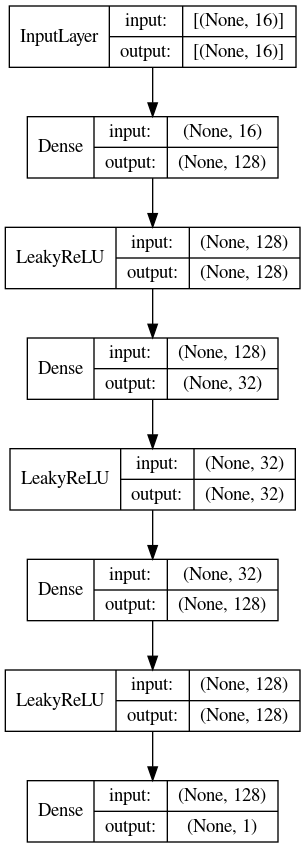
\includegraphics[width=.5\linewidth]{Plots/model_0fj.png}
    \end{subfigure}%
    \begin{subfigure}{.5\textwidth}
      \centering
      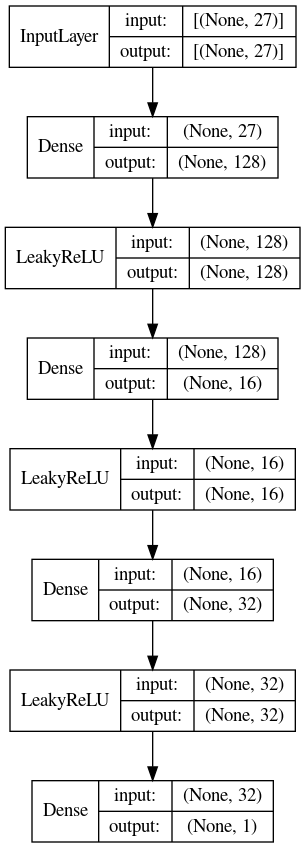
\includegraphics[width=.5\linewidth]{Plots/model_1fj.png}
    \end{subfigure}
    \caption{Plots visualizing the NN architecture for the zero forward jet region (left) and the $\geq 1$ forward jets region (right).}
    \label{fig:models}
    \end{figure}
\begin{enumerate}
    \item Newest architecture needed
    \item Formulas for ReLu and output
\end{enumerate}
\section{Input features for the neural network}

\begin{table}
    \centering
    \begin{tabular}{c|c|c}
        \toprule
        {} &                     0fj variables      & 1fj variables\\
        \midrule 
        1  &                                HT      & HT\\ \hline
        2  &                           blep\_dr     & blep\_dr\\ \hline
        3  &                           lbj\_eta     &lbj\_eta\\ \hline
        4  &                            lbj\_pt     &lbj\_pt\\ \hline
        5  &  lbj\_tagWeightBin\_DL1r\_Continuous   & lbj\_tagWeightBin\_DL1r\_Continuous\\ \hline
        6  &                          lep1\_eta     & lep1\_eta\\ \hline
        7  &                           met\_met     &met\_met\\ \hline
        8 &                             ph\_pt     &ph\_pt\\ \hline
        9 &                             top\_m     & top\_m\\ \hline
        10 &                       transMassWb      &transMassWb\\ \hline
        \midrule
        11  &                            bph\_pt     & bph\_m\\ \hline
        12 &                          topph\_pt     &topph\_ctheta\\ \hline
        13 &                            ph\_eta     & ph\_phi\\ \hline
        14 &                          lepph\_dr     & lep1\_pt\\ \hline
        15 &                      transMassWph      & met\_phi\\ \hline
        16 &                           lep1\_id     & lbj\_phi\\ \hline
        17 &&                                           Wbsn\_e \\ \hline
        18 &&                                            bfj\_m \\ \hline
        19 &&                                           blep\_m \\ \hline
        20 &&                                           fj\_eta \\ \hline
        21 &&                                           fj\_phi \\ \hline
        22 &&                                        fjet\_flag \\ \hline
        23 &&                                      fjph\_ctheta \\ \hline
        24 &&                                        fjph\_deta \\ \hline
        25 &&                                          fjph\_dr \\ \hline
        26 &&                                           fjph\_e \\ \hline
        27 &&                                           fjph\_m \\ \hline
        \bottomrule 
    \end{tabular}
    \caption{Input variables of the NN trained on events with no forward jets and the NN trained on events with at least one forward jet.}
    \label{tab:features}
\end{table}

\begin{enumerate}
    \item Where can I find the newest input feautures?
\end{enumerate}
\section{Performance and distribution of the NN output}
\begin{enumerate}
    \item Where can I find the newest input feautures?
    \item Loss function, Accuracy, Weighted Auccracy, AUC, and Weighted AUC 
    \begin{enumerate}
        \item Which plots to show and which not to show?
    \end{enumerate}
\end{enumerate}